\headline{{\textbf{\Large\sffamily Bonsai Roots:}}\\
          {\textbf{\large\sffamily Meet the Members of TWBC}}}
\label{2025-11-roots}
\noindent
In every edition of \emph{Bonsai Roots}, we pause from wiring, watering, and weekend workshops to celebrate the people who shape our club. Each story adds character to the ever\--growing forest of TWBC. This month, we're excited to introduce \textbf{Dante}!

\begin{itemize}
    \item \textbf{What's your name and where in the country do you live?}

    \emph{My name is Dante Martini and I live in Sunbury on Thames in Surrey.}

    \item \textbf{What are your favourite species of tree and why?}

    \emph{Junipers! While travelling through Japan they immediately caught my attention --- especially the shohin sizes. Their beauty, paired with the intricate shari, is what truly sparked my fascination.}

    \item \textbf{What aspect of bonsai do you enjoy?}

    \emph{I love going on walks and looking at trees, imagining what each might look like as a bonsai. Observing trees in nature is absolutely my favourite aspect.}

    \item \textbf{What aspects of bonsai do you find most challenging?}

    \emph{Interestingly, the same thing I enjoy most is also the most challenging --- envisioning what the final design of a tree will look like once it's in my hands.}

    \item \textbf{Who or what inspires you throughout your bonsai journey?}

    \emph{Coming to the club and being surrounded by like\--minded people truly inspires me. I get to talk about what I love and learn from others every time.}

    \begin{window}[2,l,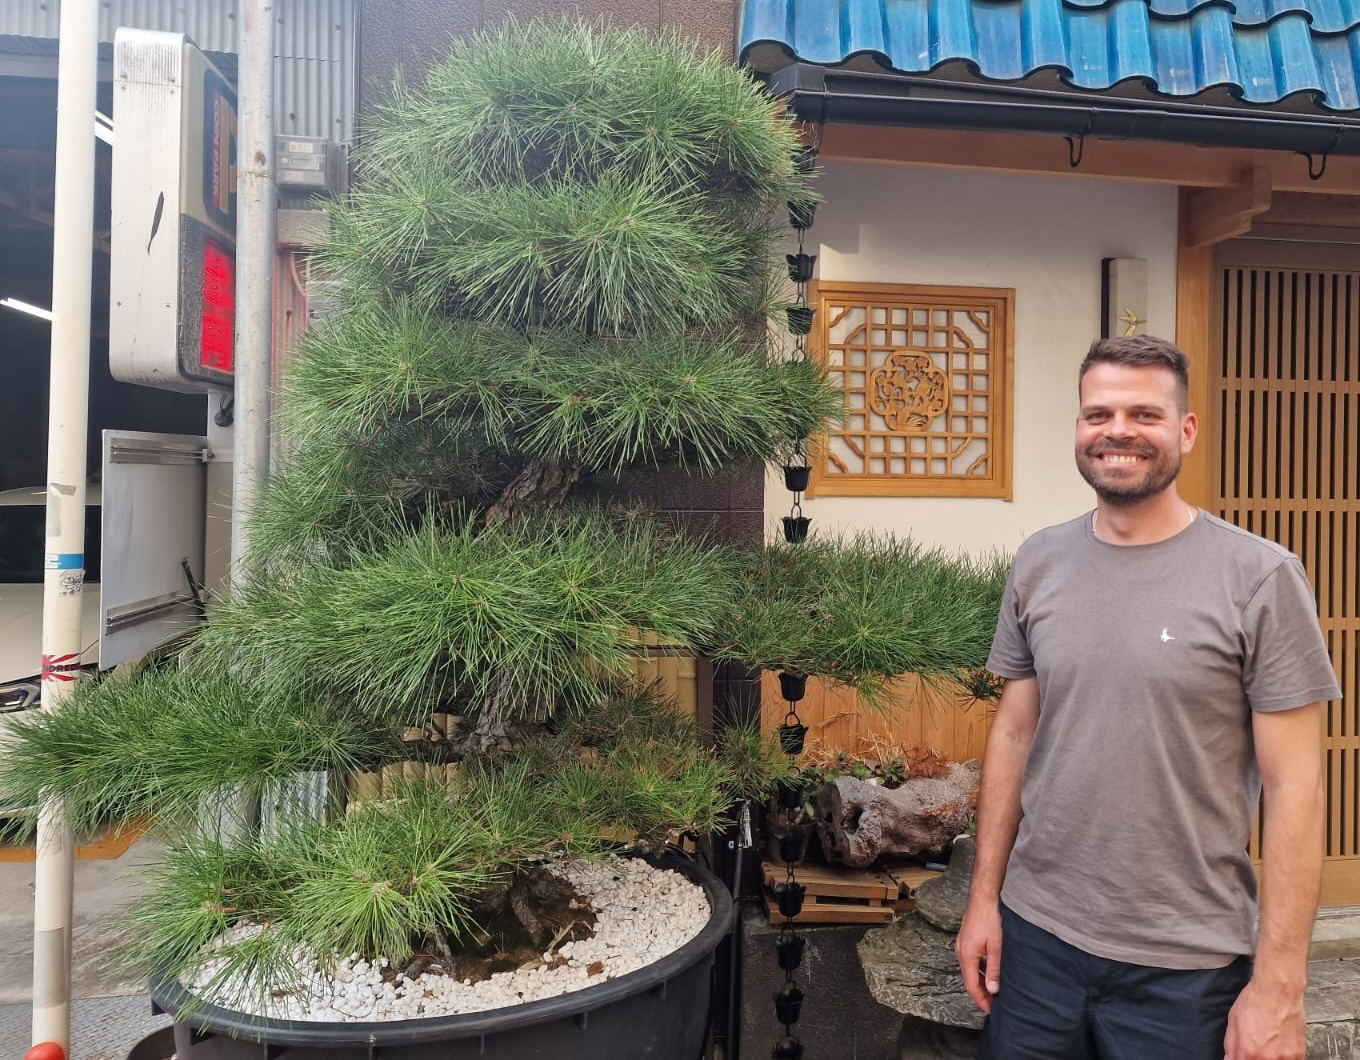
\includegraphics[width=1.0\columnwidth]{2025_11/res/roots_dante_martini.jpg},\centerline{\emph{Dante standing next an imposing pine during a trip to Japan.}}]
    \end{window}
    \columnbreak


    \item \textbf{How long have you been interested in keeping bonsai?}

    \emph{I joined my first bonsai club in South Africa at 16 years old. When I moved to the UK ten years ago, I had to pause the hobby until earlier this year.}

    \item \textbf{What stimulated your interest in bonsai?}

    \emph{Returning to Japan this year reignited everything --- buying tools, seeing bonsai everywhere, it all brought that passion back to life.}

    \item \textbf{If you could give someone new to bonsai any tips, what would it be?}

    \emph{Just start! You don't need all the tools or expertise. Join a club and be part of the community --- the rest will follow.}

    \item \textbf{Why do you enjoy being part of TWBC, and do you have any ideas or suggestions for the club's future?}

    \emph{Every time I'm at TWBC I learn something new from someone. That sense of shared knowledge is invaluable.}

    \item \textbf{One word to describe what bonsai means to you?}

    \emph{Peace.}

    \item \textbf{What are your future goals regarding your own trees and learning more about the hobby?}

    \emph{One day, I'd love to have one of my trees displayed in an exhibition.}

    \item \textbf{How would you like to see your bonsai journey progress in the future?}

    \emph{I hope to gain more confidence and experience so I can work on trees without hesitation or doubt.}
\end{itemize}

Dante's bonsai story is one of rediscovery, inspiration, and growing confidence --- a journey rooted in passion and guided by community. We can't wait to see his trees and skills continue to develop. Who will we meet next time? Stay tuned for more in \emph{Bonsai Roots}!

\begin{center}
$\cdots$
\end{center}

\noindent
\emph{If you're a newer member and would like to feature in a future edition of Bonsai Roots, simply fill out the form at \href{https://forms.gle/quVXa4L8rhpnT5kr6}{this link}! We'd love to hear your story.}

\closearticle
\columnbreak